% \input{\pSections fig-geometry}

% nb: /Users/dantopa/Mathematica_files/nb/projects/hii-tsd/orbits/kepler/ellipse-01.nb
\begin{figure}[htbp] %  figure placement: here, top, bottom, or page
   \centering
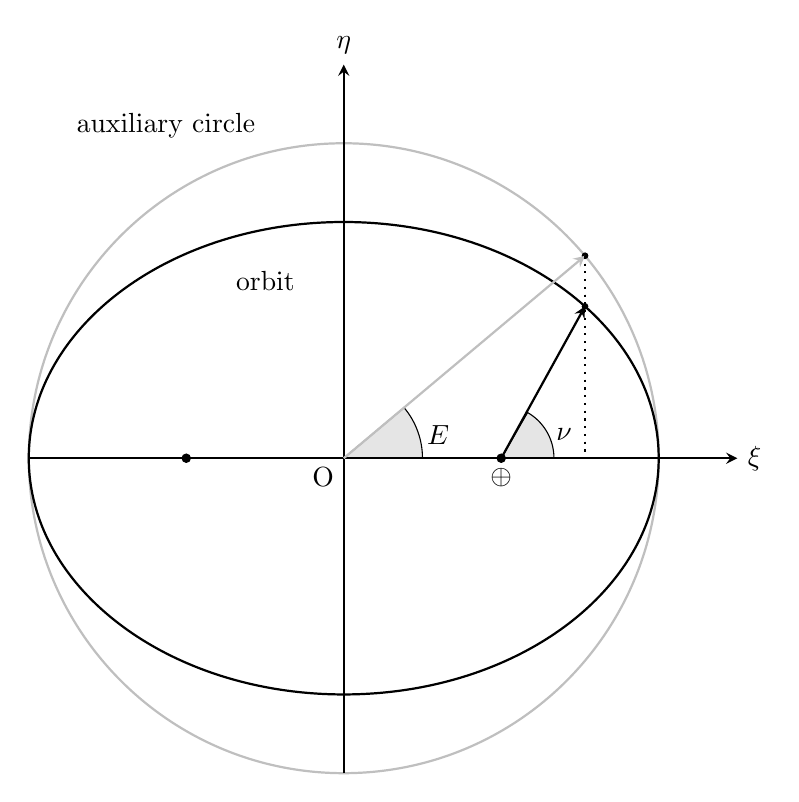
\begin{tikzpicture}

    % Define parameters
    \def\radius{4} % Radius of the circle
    \def\angle{40} % Angle theta (pi/6) in degrees
    \def\focusX{2} % Focus of the ellipse (positive x-axis)
    \def\semiMajor{4} % Semi-major axis of the ellipse
    \def\semiMinor{3} % Semi-minor axis of the ellipse

    % Shaded angle for POp (angle = theta)
    \filldraw[ fill=gray!20 ] (0,0) -- (1,0) arc[start angle=0, end angle=\angle, radius=1cm] -- cycle;
    \node at (1.2, 0.3) {$E$};

    % Shaded angle for Pfq (angle subtended by Pfq)
    %\filldraw[ fill=gray!20 ] (\focusX, 0) -- ++(0.67,0) arc[start angle=0, end angle=\angle, radius=0.67cm] -- cycle;
    \filldraw[ fill=gray!20 ] (\focusX, 0) -- ++(0.67,0) arc[start angle=0, end angle=60, radius=0.67cm] -- cycle;
    \node at (2.8, 0.3) {$\nu$};

    % Circle (gray)
    \draw[ thick, gray!50 ] (0,0) circle(\radius cm);

    % Ellipse (black)
    \draw[ thick, black ] (0,0) ellipse (\semiMajor cm and \semiMinor cm);

    % Axes
    \draw[ ->, thick, -stealth ] (-\radius,0) -- (5,0) node[anchor=west] {$\xi$}; % Horizontal axis
    \draw[ ->, thick, -stealth ] (0,-\radius) -- (0,5) node[anchor=south] {$\eta$}; % Vertical axis

    % Origin (O)
    \node at (0,0) [ below left ] {O};
    %\node at (\focusX, -0.3) {f};

    % Point P on the circle (corresponding to theta = pi/6)
    \coordinate (P) at ({\radius*cos(\angle)}, {\radius*sin(\angle)});
    \filldraw (P) circle(1pt);% node[anchor=south west] {P};

    % Point Q on the ellipse (Q = (a cos theta, b sin theta))
    \coordinate (Q) at ({\semiMajor*cos(\angle)}, {\semiMinor*sin(\angle)});
    \filldraw (Q) circle(1pt);% node[anchor=north east] {Q};

    % Arrow from O to P (Op) with tail at the origin and head at P
    \draw[ ->, thick, -stealth, gray!50 ] (0,0) -- (P) node[midway, above right] {};

    % Arrow from f to Q (fq) with tail at the focus and head at Q
    \draw[ ->, thick, -stealth ] (\focusX, 0) -- (Q) node[midway, below right] {};

    % Dotted line from P to Q
    \draw[dotted, thick] (P) -- (Q);

    % Dotted line from P to the horizontal axis
    \draw[dotted, thick] (P) -- ({\radius*cos(\angle)}, 0);

    % Earth symbol at positive focus (f) with white background
    %\node[ fill=white ] at (\focusX, 0) {$\oplus$};
    %\node[ fill=none ] at (\focusX, 0) {$\oplus$};

    % Mark the other focus (negative focus)
    \filldraw (-\focusX,0) circle(1.5pt);% node[below left] {Focus};
    \filldraw (\focusX,0) circle(1.5pt) node[ below ] {$\oplus$};

    \node at (-1,4.5) [ below left ] {auxiliary circle};
    \node at (-0.5,2.5) [ below left ] {orbit};

\end{tikzpicture}
   \caption{Orbit trajectory (black) and the auxiliary circle (gray) showing the angles for eccentric anomaly, $E$, and the true anomaly, $\nu$. The true anomaly indicates position relative to the Earth, $\oplus$, while the eccentric anomaly points to an echo point on the auxiliary circle.}
   \label{fig:geometry}
\end{figure}
